\documentclass[10pt,conference]{IEEEtran}

\usepackage{cite}
\usepackage{amsmath,amssymb,amsfonts}
\usepackage{algorithmic}
\usepackage{graphicx}
\usepackage{textcomp}
\usepackage{xcolor}
\def\BibTeX{{\rm B\kern-.05em{\sc i\kern-.025em b}\kern-.08em
    T\kern-.1667em\lower.7ex\hbox{E}\kern-.125emX}}
\begin{document}

\title{Automatically Generating Follow-up Questions for Incomplete Bug Reports}

\author{\IEEEauthorblockN{1\textsuperscript{st} Given Name Surname}
\IEEEauthorblockA{\textit{dept. name of organization (of Aff.)} \\
\textit{name of organization (of Aff.)}\\
City, Country \\
email address or ORCID}
\and
\IEEEauthorblockN{2\textsuperscript{nd} Given Name Surname}
\IEEEauthorblockA{\textit{dept. name of organization (of Aff.)} \\
\textit{name of organization (of Aff.)}\\
City, Country \\
email address or ORCID}
\and
\IEEEauthorblockN{3\textsuperscript{rd} Given Name Surname}
\IEEEauthorblockA{\textit{dept. name of organization (of Aff.)} \\
\textit{name of organization (of Aff.)}\\
City, Country \\
email address or ORCID}
}

\maketitle

\begin{abstract}
This document is
\end{abstract}

\begin{IEEEkeywords}
component, formatting, style, styling, insert
\end{IEEEkeywords}

\section{Introduction}

In many popular software projects, bug reports arrive with frequency and in bursts that can overwhelm even well-resourced and well-organized bug triage.
%
At the same time, numerous bug reports lack sufficient actionable information for bug triagers to reproduce the bug.
%
Practitioners and researchers have observed this problem of bug report inadequacy, reporting that over 60\% of bug reports lack any steps to reproduce and over 40\% lack any description of the expected behavior~\cite{chaparro17detecting}.
%
While some software projects publish bug reporting guidelines (e.g., specific templates bug reports must follow), there are many cases where such guidelines are not followed and numerous cases where bug reports still lack crucial context or detail.
%
Bug triagers posing quick follow up questions in order to elicit additional information from bug reporters is one method to augment the bug reports with necessary information.
%
However follow-up questions are only effective if they are posed quickly, before the bug reporter loses focus on the specific bug.
%
In this paper, we examine how the posing such follow-up questions for inadequate bug reports can be performed automatically, designing and describing a system to reduce bug triage effort and improving overall bug report quality by automatically posing follow-up questions for inadequate bug reports.

\begin{figure}[ht]
\centering
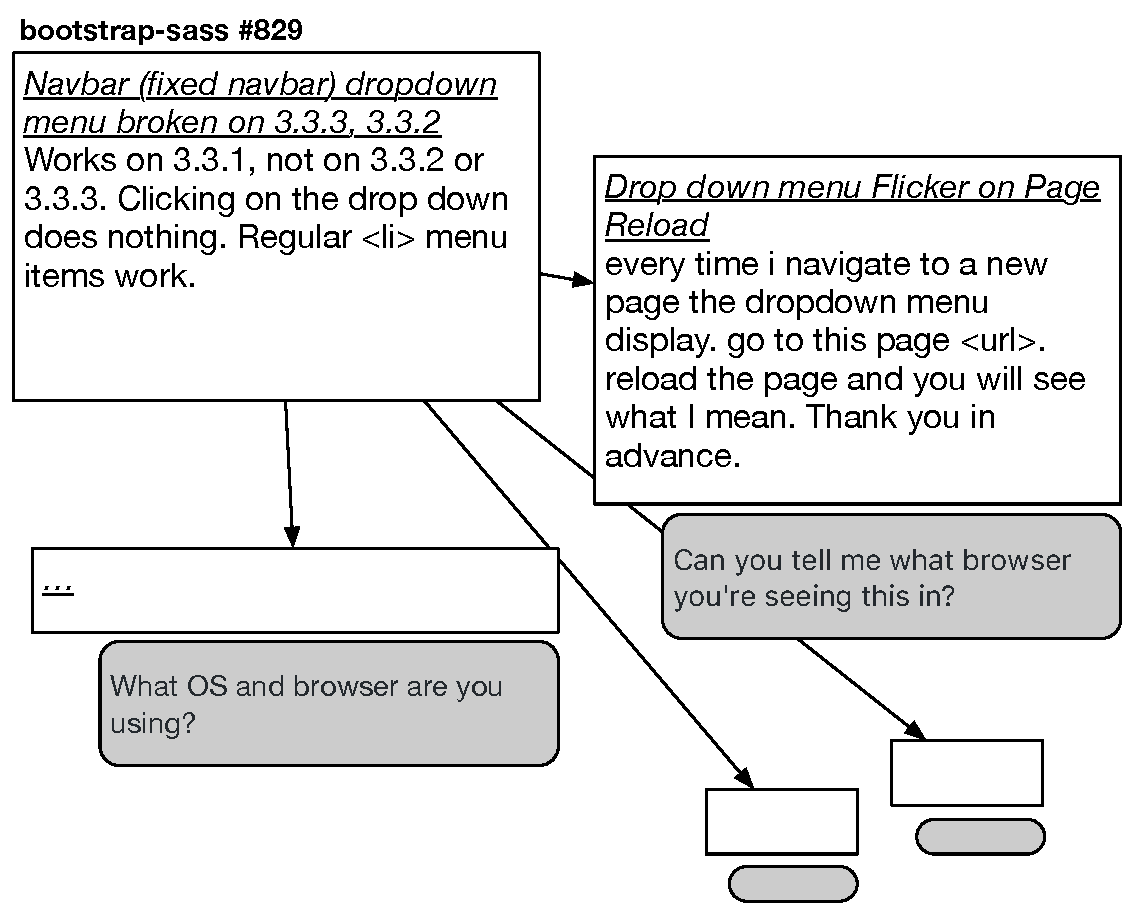
\includegraphics[width=0.99\linewidth]{figures/br_motivation.pdf}
\caption{The text for bug report (\#829) of the bootstrap-sass project is similar to other bug reports with posed follow-up questions. These follow-up questions could be recommended for this bug report.}
\label{fig:repo_activity}
\end{figure}


%
We base our automatic follow-up question posing system on the idea that: 1) relevant follow-up question are common and have already been posed in other prior bug reports, in the current project or in others; 2) similar bug reports necessitate similar follow-up questions; and 3) the utility of the answer provided to a prior similar follow up question is indicative of its value to the current bug report.
%
Therefore the task our system performs is to retrieve the most relevant and useful follow-up question for a specific inadequate bug report, given a large corpus of previous bug reports, follow-up questions, and their answers.
%
For instance, consider the example shown in Figure 1, where the bug report ....

To curate a corpus of prior bug reports, follow-up questions, and answers we leverage GitHub, where we focus on popular repositories that have a high level of activity and therefore a likely to have utilized the follow-up questions mechanism. We look for follow-up questions that have been posed in comments and gather answers that occur as comments or as edits to the original bug report text. To estimate the utility of an answer we use the patterns to identify Observable Behavior (OB), Expected Behavior (EB) and Steps to Reproduce (S2R), published by Chaparro et al. We evaluate our prototype in two ways, based on the ability to predict an annotated held-out set of follow-up questions, and based on a developer survey that aims to gage the perceived value of specific follow up questions. The results indicate that the techniques is viable, with X MRR on the held-out set and Y\% of respondents indicating that the follow-up question is “bla bla bla”.

Relative to the prior efforts by the software engineering research community towards improving the quality of bug reports, this paper is the first to use follow-up questions and to propose a specific mechanism for this purpose. Automatically posing follow-up has been used in other domains for improving the quality of Web forum posts~\cite{rao-daume-iii-2018-learning}, product reviews in online retail, and improving query quality in Web search.

% More specifically, the contributions of this paper are:
%
% \begin{itemize}
% \item x
% \item y
% \item z
% \end{itemize}


\section{Bug Reporting in Open Source Projects}


%The problem is real, i.e., there are repos that have more BRs than they can manage. How many BRs arrive at the most popular repos (is the traffic bursty)? how many lack OB/EB/S2R from these?
The overall trend in software development in recent years is towards increased
speed of development and delivery. There are nowadays numerous projects on popular
public software collaboration platforms like GitHub that have large development
teams and user communities. Many of these projects experience significant
bug reporting traffic~\cite{Zhang2014ASO}. Figure~\ref{fig:repo_activity} shows the issue creation
frequency for a selection of ten GitHub repositories that are currently active
with a high numbers of commits and developers. Three of these repositories have
a median of over 40 issues created daily, where most of them are bug reports reported by
GitHub identities that have not contributed to the project (i.e., users). In addition,
the same three projects exhibit high variance in daily issue creation, likely indicative
of bursty and hard to predict bug reporting activity. This is a
considerable burden for bug triagers and it motivates the need for the type of work
as described in this paper, which intends to make bug triage more efficient and less of
a burden for project maintainers.


\begin{figure}[t]
\centering
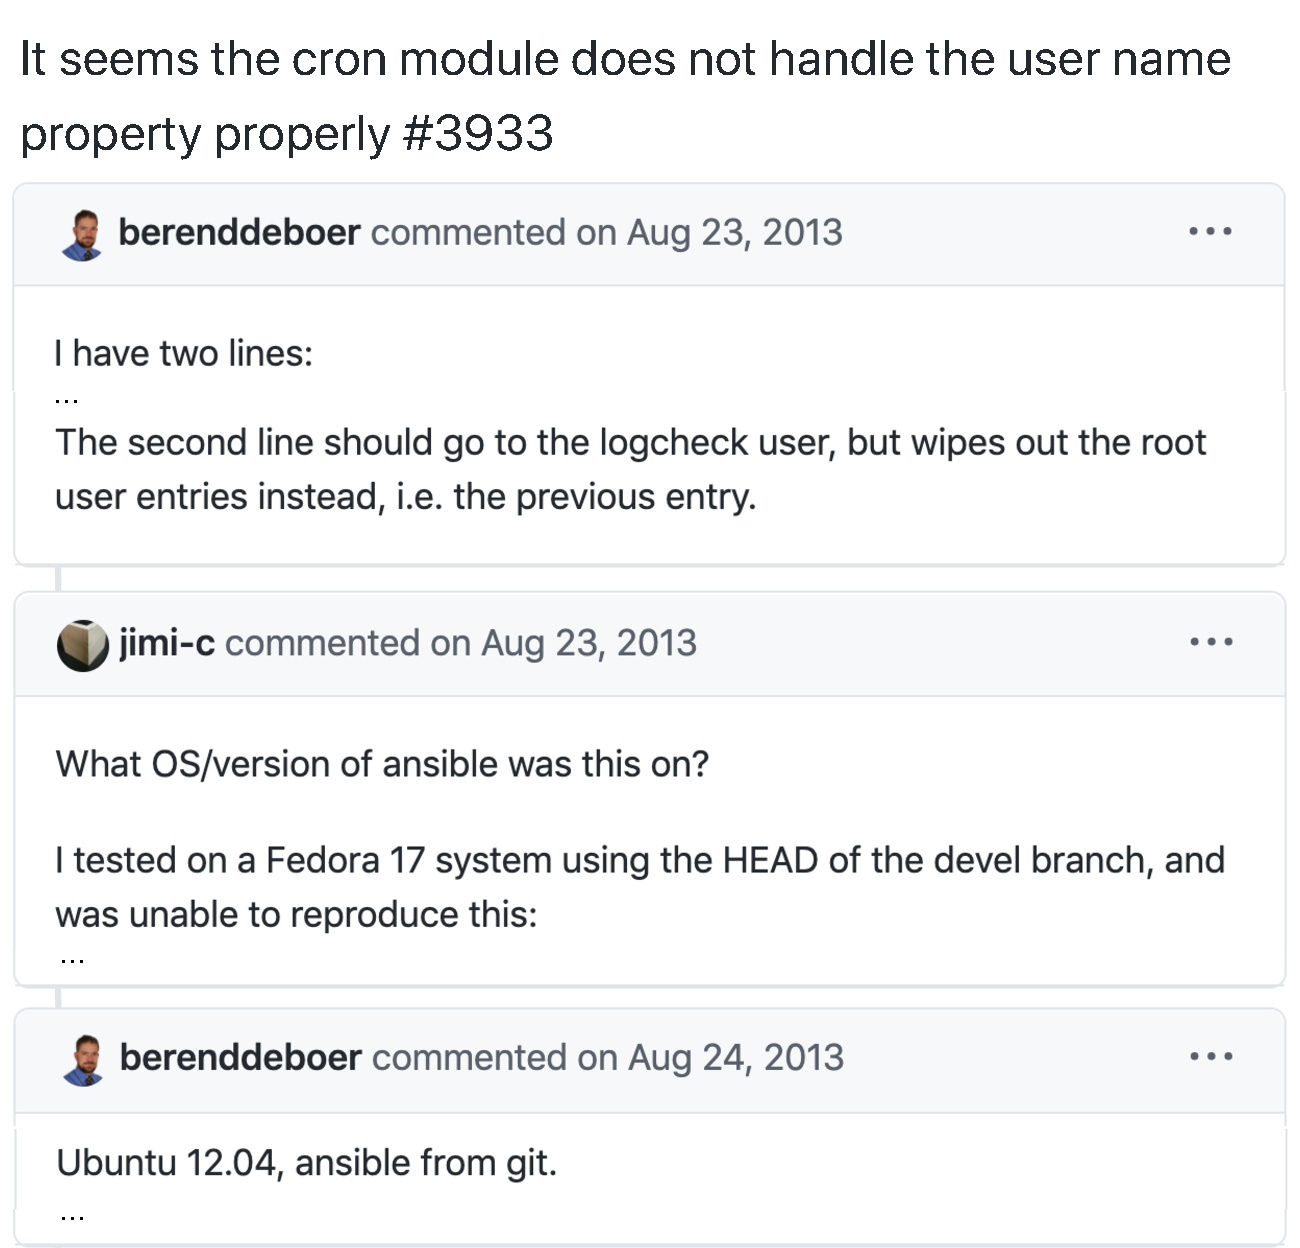
\includegraphics[width=0.99\linewidth]{figures/bug_report.pdf}
\caption{Bug report with follow-up question and OB in answer.}
\label{fig:bug_report}
\end{figure}

% The preconditions are present, i.e., there are a lot of follow-up questions on GitHub -- we could
% use the same set of 10 repos to show this.
Posing follow-up questions is an already practiced mitigation strategy for deficient bug
reports. To lend support for this claim and to quantify how widespread is the use of
follow-up questions, we performed a small scale study of the prevalence
of follow-up questions on GitHub, focusing on the 10 active projects used in Figure~\ref{fig:repo_activity}.
From each of the 10 repositories, we randomly sampled 50 closed bug reports (500 in total) and manually examined them
for follow-up questions. We were also interested whether the answers to those questions (if they are present) provide any
of the three key parts of a bug report: Observable Behavior (OB), Expected Behavior (EB) or Steps to Reproduce (S2R).
We found that follow-up questions were present in 23.6\% (118/500) of bug reports and about 73\% (86/118) of them were
answered with 57\% (49/86) of the answers containing Observable Behavior, Expected Behavior or Steps to Reproduce.

We highlight one of the bug reports we examined ({\bf ansible/ansible \#3933}) in Figure~\ref{fig:bug_report}. The follow-up question {\em What OS/version of
Ansible was this on?} elicited an answer that provided key OB to this bug report, leading to its quick subsequent fix.
Developer surveys have confirmed the importance of OB, EB and S2R in bug reports , noting that S2R is among the most valuable aspects of a bug report
with OB and EB closely behind~\cite{zimmermann10whatmakes,laukkanen2011survey}. The availability of existing follow-up questions on social coding platforms like GitHub provides the preconditions for the approach described in this paper, which leverages such existing follow-up questions to automatically rank and select the most appropriate one to be asked for a newly written, incomplete bug report. In the remainder of this paper, we describe the design of this system, which we entitle \evpi\ -- Bug Incompleteness Questioner\footnotemark\footnotetext{Replication package available at: https://tinyurl.com/y223uva2}.


\section*{Acknowledgment}

Something goes here

\bibliographystyle{IEEEtran}
\bibliography{paper}

\end{document}
